\chapter{Geometry creation}\label{chap:GeometryCreation}
The creation of geometry objects within the computational domain is
a crucial part of the simulation process.  This chapter discusses the
options avialble for creating geometry in \Vaango.

\section{Basic geometry objects} \label{Sec:GeometryObjects}

Each geometry object has the following properties, label (string
name), type (box, cylinder, sphere, etc), resolution (vector
quantity), and any unique geometry parameters such as origin, corners,
triangulated data file, etc.  The operators which include, the union,
the difference, and intersection tags contain either lists of
additional operators or the primitives pieces.

As an example of a non-trivial geometry object is shown below:

\begin{lstlisting}[language=XML]
<geom_object>
     <intersection>
       <box label = "Domain">
          <min>[0.0,0.0,0.0]</min>
          <max>[0.1,0.1,0.1]</max>
       </box>
       <union>
         <sphere label = "First node">
            <origin>[0.022,0.028,0.1  ]</origin>
            <radius>0.01</radius>
         </sphere>
         <sphere label = "2nd node">
            <origin>[0.030,0.075,0.1  ]</origin>
            <radius>0.01</radius>
         </sphere>
       </union>
     </intersection>
     <res>[2,2,2]</res>
     <velocity>[0.,0.,0.]</velocity>
     <temperature>0 </temperature>
</geom_object>
\end{lstlisting}

The following geometry objects are given with their required tags:

\subsection{Box}
\begin{minipage}{0.6\textwidth}
  \Textsfc{box} requires the tags \Textsfc{min} and \Textsfc{max} which are
  vector quantities specified in the \Textsfc{[a, b, c]} format.
  \begin{lstlisting}[language=XML]
    <box label="box_1">
      <min>[0.0, 0.0, 0.0]</min>
      <max>[1.0, 2.0, 3.0]</max>
    </box>
  \end{lstlisting}
\end{minipage}
\begin{minipage}{0.4\textwidth}
  \centering
  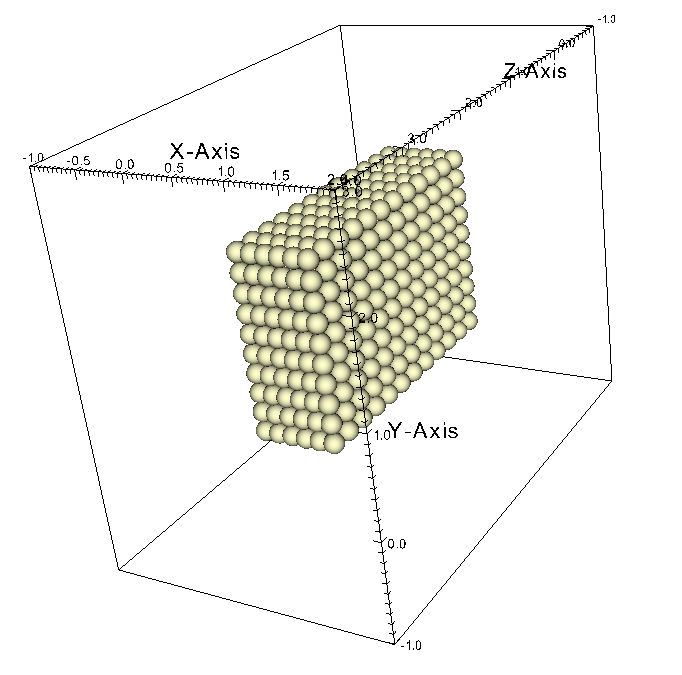
\includegraphics[width=0.9\columnwidth]{FIGS/geometry/geom_box.png}
  \captionof{figure}{A \Textsfc{box} geometry piece.}
\end{minipage}

\subsection{Parallelepiped}
\begin{minipage}{0.6\textwidth}
  \Textsfc{parallelepiped} requires the locations of four points
  that define the bounds of the parallelepiped.  The point \Textsfc{p1}
  is a corner while the the vectors \Textsfc{p2 - p1}, \Textsfc{p3 - p1},
  and \Textsfc{p4 - p1} represent the vectors along the three edges
  of the parallelepiped starting from \Textsfc{p1}.
  \begin{lstlisting}[language=XML]
    <parallelepiped label="box_1">
      <p1>[ 0.0, 0.0, 0.0]</p1>
      <p2>[ 1.0, 0.0, 0.0]</p2>
      <p3>[ 1.0, 2.0, 0.5]</p3>
      <p4>[-1.0, 1.0, 2.0]</p4>
    </parallelepiped>
  \end{lstlisting}
  \centering
  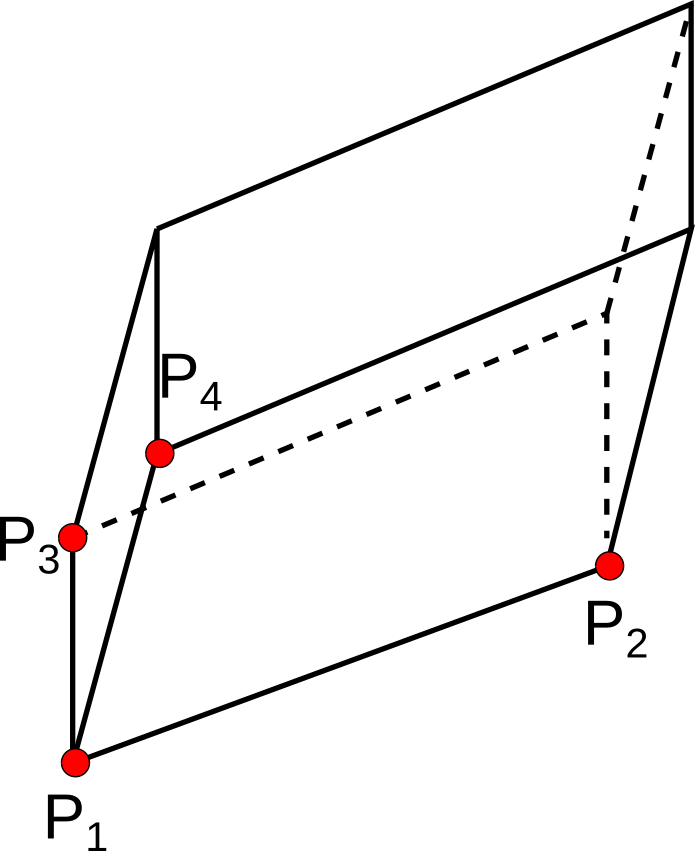
\includegraphics[width=0.3\columnwidth]{FIGS/geometry/naa_box_def.png}
\end{minipage}
\begin{minipage}{0.4\textwidth}
  \centering
  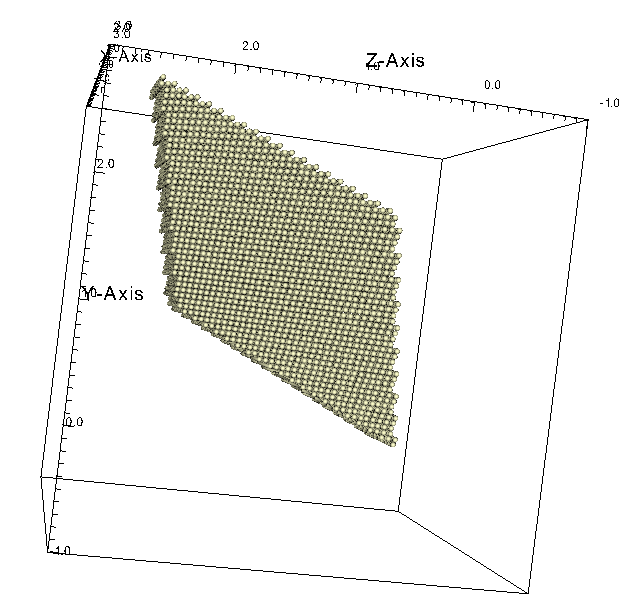
\includegraphics[width=0.9\columnwidth]{FIGS/geometry/geom_naa_box.png}
  \captionof{figure}{A \Textsfc{parallelepiped} geometry piece.}
\end{minipage}

\subsection{Sphere}
\begin{minipage}{0.6\textwidth}
  \Textsfc{sphere} has an \Textsfc{origin} tag specified as a vector and the
  \Textsfc{radius} tag specified as a float.
  \begin{lstlisting}[language=XML]
    <sphere label="ball_1">
      <origin>[ 0.0, 0.0, 0.0]</origin>
      <radius> 0.75 </radius>
    </sphere>
  \end{lstlisting}
\end{minipage}
\begin{minipage}{0.4\textwidth}
  \centering
  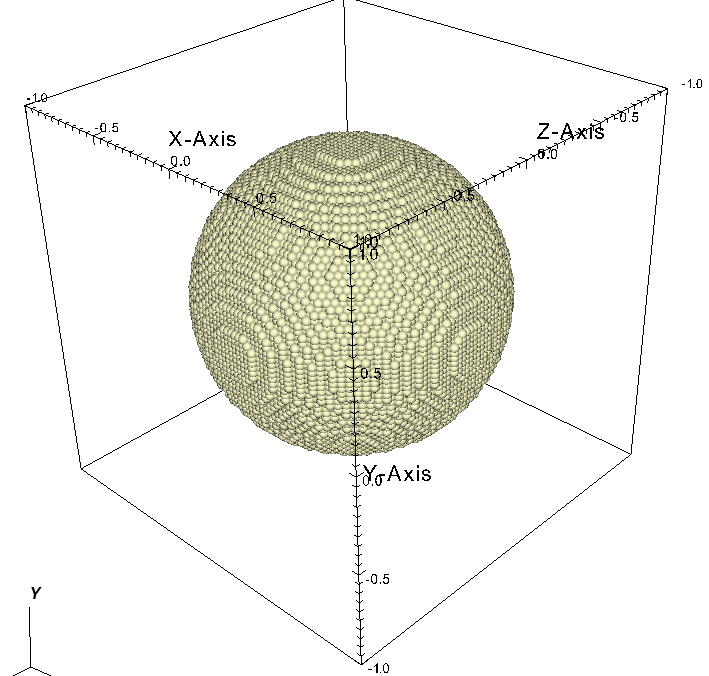
\includegraphics[width=0.9\columnwidth]{FIGS/geometry/geom_sphere.png}
  \captionof{figure}{A \Textsfc{sphere} geometry piece.}
\end{minipage}

\subsection{Cylinder}
\begin{minipage}{0.6\textwidth}
  \Textsfc{cylinder} has a tag for the \Textsfc{top} and \Textsfc{bottom} origins
  (vector) plus a tag for the \Textsfc{radius} (float).
  \begin{lstlisting}[language=XML]
    <cylinder label="cyl_1">
      <bottom>[ -0.5, -0.5, -0.5]</bottom>
      <top>[ 1.5, 1.5, 1.5]</top>
      <radius> 0.5 </radius>
    </cylinder>
  \end{lstlisting}
\end{minipage}
\begin{minipage}{0.4\textwidth}
  \centering
  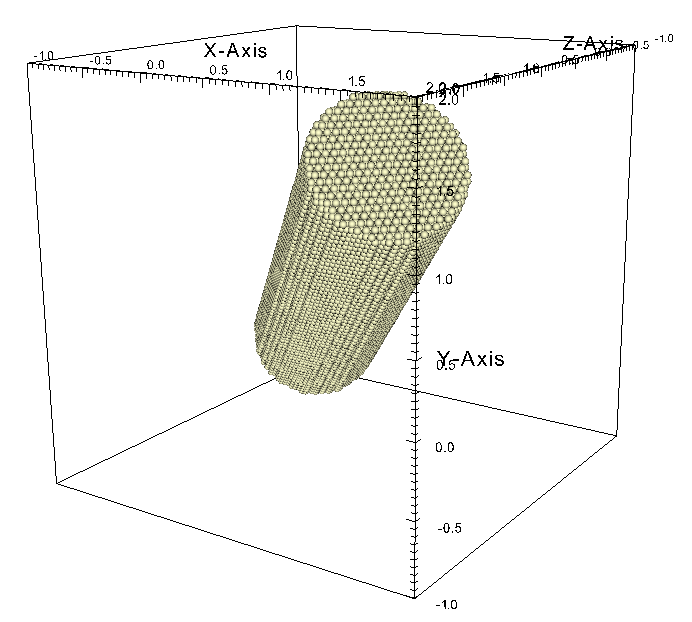
\includegraphics[width=0.9\columnwidth]{FIGS/geometry/geom_cyl.png}
  \captionof{figure}{A \Textsfc{cylinder} geometry piece.}
\end{minipage}

\subsection{Cone}
\begin{minipage}{0.6\textwidth}
  \Textsfc{cone} has a tag for the \Textsfc{top} and \Textsfc{bottom} origins (vector)
  as well as tags for the top and bottom \Textsfc{radius} (float) to create a
  right circular cone/frustum.
  \begin{lstlisting}[language=XML]
    <cone label="cone_1">
      <bottom>[ -0.5, -0.5, -0.5]</bottom>
      <top>[ 1.5, 1.5, 1.5]</top>
      <bottom_radius> 0.7 </bottom_radius>
      <top_radius> 0.1 </top_radius>
    </cone>
  \end{lstlisting}
\end{minipage}
\begin{minipage}{0.4\textwidth}
  \centering
  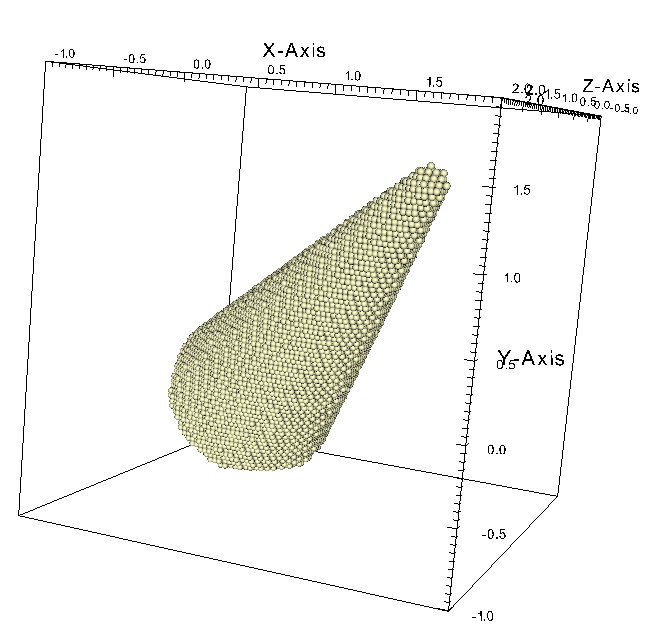
\includegraphics[width=0.9\columnwidth]{FIGS/geometry/geom_cone.png}
  \captionof{figure}{A \Textsfc{cone} geometry piece.}
\end{minipage}

\subsection{Ellipsoid}
\begin{minipage}{0.6\textwidth}
  \Textsfc{ellipsoid} has an \Textsfc{origin} tag specified as a vector.  
  An ellipsoid is defined by two orthogonal axis vectors \Textsfc{v1} and
  \Textsfc{v2} and three semi-axis lengths \Textsfc{r1}, \Textsfc{r2}, \Textsfc{r3}.
  The axis vectors must be orthogonal to within 1e-12 after dot product or 
  the simulation will throw an exception.  
  \begin{lstlisting}[language=XML]
    <ellipsoid label="ellipsoid_1">
      <origin>[ 0.0, 0.0, 0.0]</origin>
      <v1> [0.353553, 0.353553, 0.4] </v1>
      <v2> [0.087038295569, -0.783349583783, 0.615457362205] </v2>
      <r1> 0.6403119924052649 </r1>
      <r2> 1.0 </r2>
      <r3> 2.0 </r3>
    </ellipsoid>
  \end{lstlisting}
\end{minipage}
\begin{minipage}{0.4\textwidth}
  \centering
  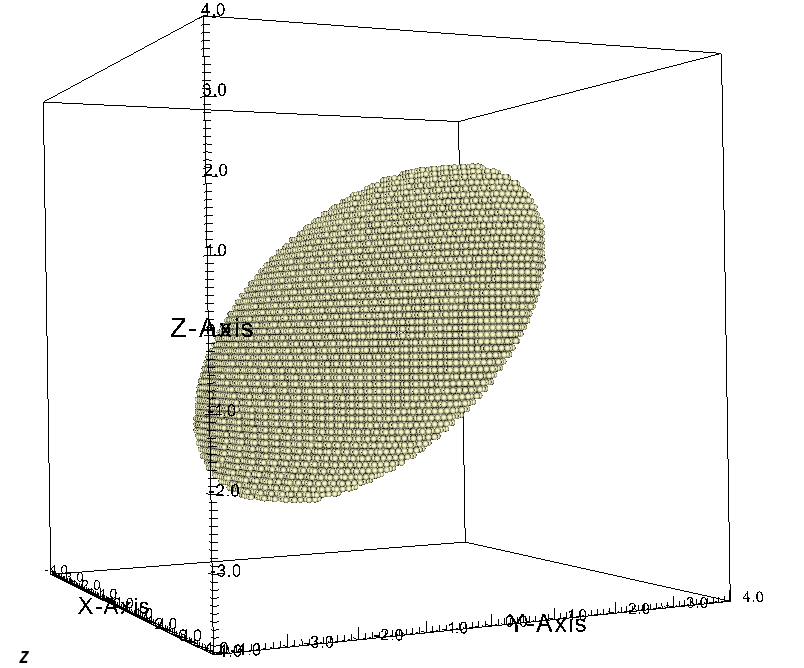
\includegraphics[width=0.9\columnwidth]{FIGS/geometry/geom_ellipsoid.png}
  \captionof{figure}{An \Textsfc{ellipsoid} geometry piece.}
\end{minipage}

\subsection{Torus}
\begin{minipage}{0.6\textwidth}
  \Textsfc{torus} has a \Textsfc{center}, an \Textsfc{axis} vector,
  and \Textsfc{major} and \Textsfc{minor} radii.   The major radius must
  be greater than the minor radius.  The axis vector is converted
  internally into a unit vector and cannot have zero length.
  \begin{lstlisting}[language=XML]
    <torus label="torus object">
      <center> [0.1, 0.1, 0.1] </center>
      <axis_vector>[ 1.5, 1.5, 1.5] </axis_vector>
      <major_radius> 1.0 </major_radius>
      <minor_radius> 0.5 </minor_radius>
    </torus>
  \end{lstlisting}
\end{minipage}
\begin{minipage}{0.4\textwidth}
  \centering
  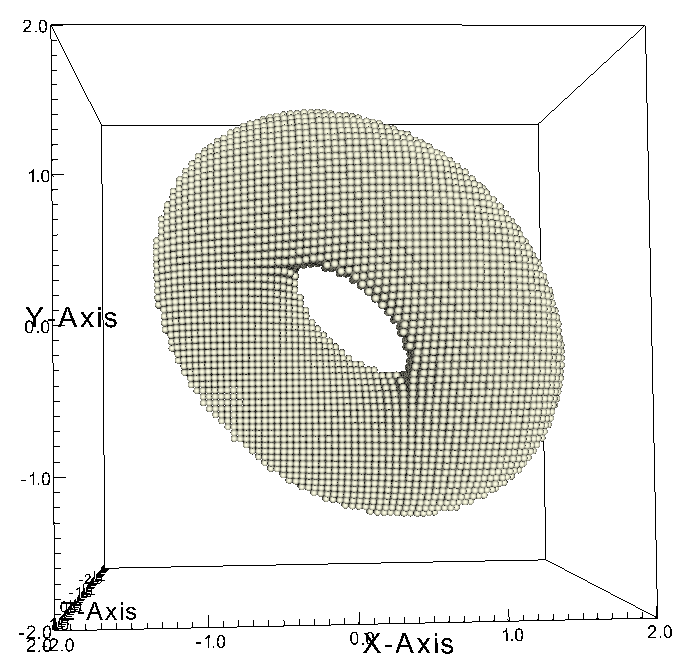
\includegraphics[width=0.9\columnwidth]{FIGS/geometry/geom_torus.png}
  \captionof{figure}{A \Textsfc{torus} geometry piece.}
\end{minipage}

\subsection{Boolean operations}
The boolean operators on the geometry pieces include \Textsfc{difference,
intersection,} and \Textsfc{union}.
Multiple operators can be used to form very complex geometry pieces.

\begin{minipage}{0.6\textwidth}
  The \Textsfc{difference} takes two geometry pieces and subtracts
  the second geometry piece from the first geometry piece.  
  \begin{lstlisting}[language=XML]
    <difference>
      <box label="box_1">
        <min>[-0.75, -0.75, -0.75]</min>
        <max>[ 0.75,  0.75,  0.75]</max>
      </box>
      <sphere label="ball_1">
        <origin>[ 0.0, 0.0, 0.0]</origin>
        <radius> 1.00 </radius>
      </sphere>
    </difference>
  \end{lstlisting}
  \begin{lstlisting}[language=XML]
    <difference>
      <sphere label="ball_1">
        <origin>[ 0.0, 0.0, 0.0]</origin>
        <radius> 1.00 </radius>
      </sphere>
      <box label="box_1">
        <min>[-0.75, -0.75, -0.75]</min>
        <max>[ 0.75,  0.75,  0.75]</max>
      </box>
    </difference>
  \end{lstlisting}
\end{minipage}
\begin{minipage}{0.4\textwidth}
  \centering
  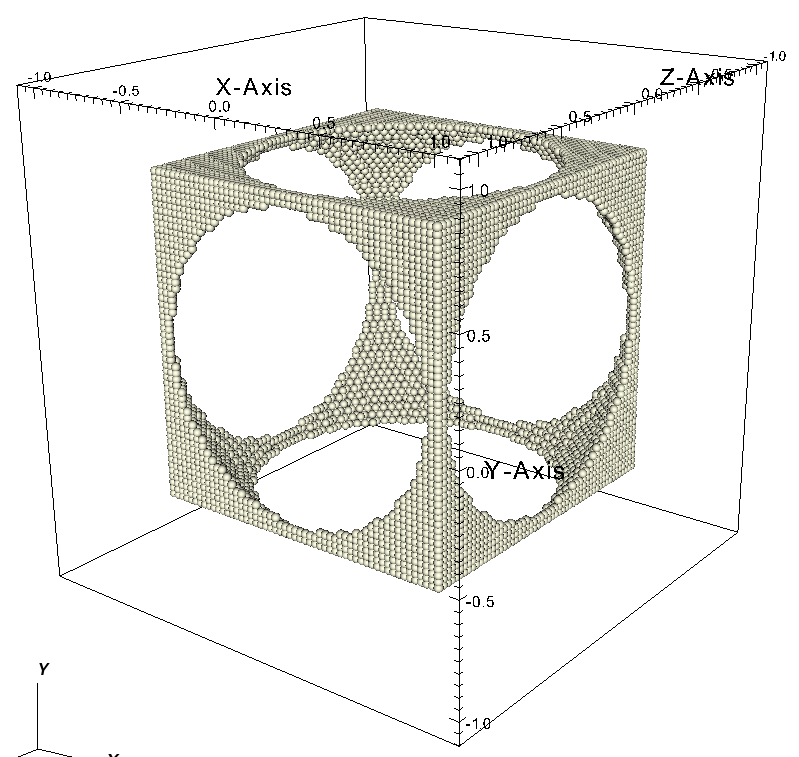
\includegraphics[width=0.9\columnwidth]{FIGS/geometry/geom_diff_12.png}
  \captionof{figure}{The \Textsfc{difference} of a sphere from a cube.}
  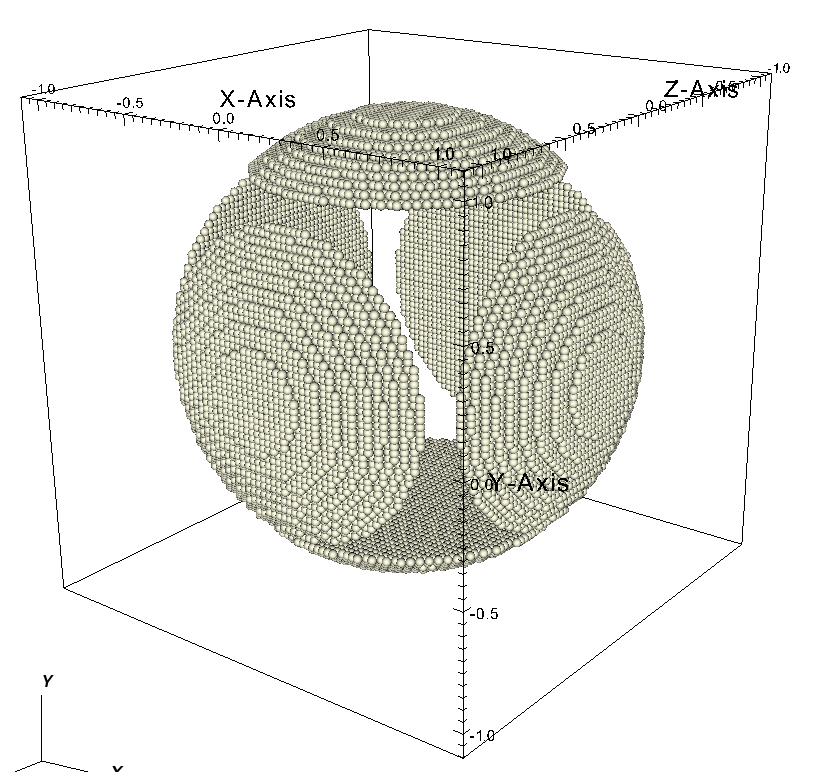
\includegraphics[width=0.9\columnwidth]{FIGS/geometry/geom_diff_21.png}
  \captionof{figure}{The \Textsfc{difference} of a cube from a sphere.}
\end{minipage}

\begin{minipage}{0.6\textwidth}
  The \Textsfc{intersection} operator requires at least two geometry
  pieces in forming an intersection geometry piece.  
  \begin{lstlisting}[language=XML]
    <intersection>
      <box label="box_1">
        <min>[-0.75, -0.75, -0.75]</min>
        <max>[ 0.75,  0.75,  0.75]</max>
      </box>
      <sphere label="ball_1">
        <origin>[ 0.0, 0.0, 0.0]</origin>
        <radius> 1.00 </radius>
      </sphere>
    </intersection>
  \end{lstlisting}
\end{minipage}
\begin{minipage}{0.4\textwidth}
  \centering
  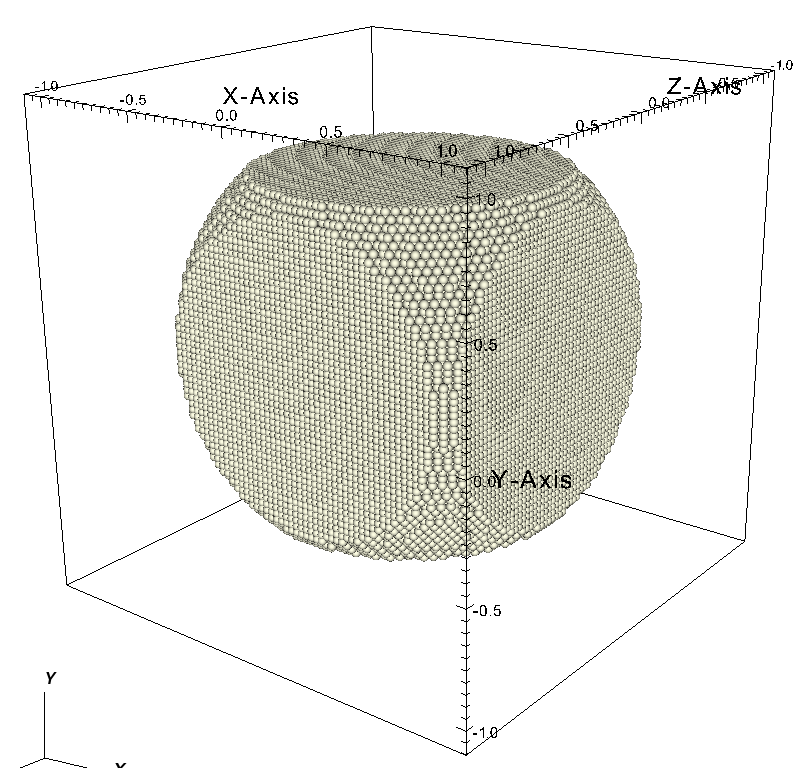
\includegraphics[width=0.9\columnwidth]{FIGS/geometry/geom_intersect.png}
  \captionof{figure}{An \Textsfc{intersection} of a sphere and a cube.}
\end{minipage}

\begin{minipage}{0.6\textwidth}
  The \Textsfc{ union} operator aggregates a collection of geometry pieces.
  \begin{lstlisting}[language=XML]
    <union>
      <box label="box_1">
        <min>[-0.75, -0.75, -0.75]</min>
        <max>[ 0.75,  0.75,  0.75]</max>
      </box>
      <sphere label="ball_1">
        <origin>[ 0.0, 0.0, 0.0]</origin>
        <radius> 1.00 </radius>
      </sphere>
    </union>
  \end{lstlisting}
\end{minipage}
\begin{minipage}{0.4\textwidth}
  \centering
  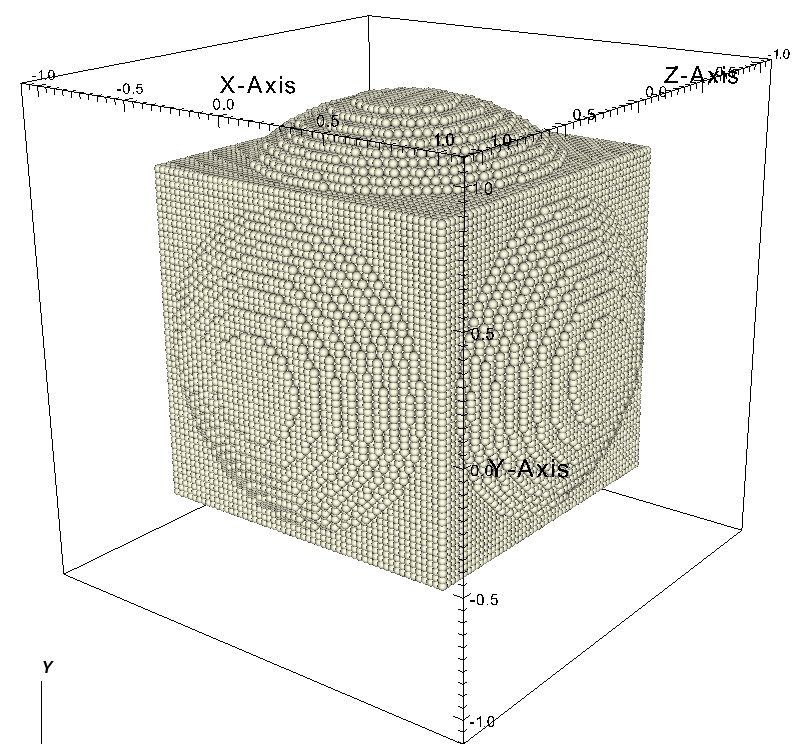
\includegraphics[width=0.9\columnwidth]{FIGS/geometry/geom_union.png}
  \captionof{figure}{A \Textsfc{union} of a sphere and a cube.}
\end{minipage}

\section{Special geometry objects} \label{Sec:SpecialGeometryObjects}
A few special geometry objects exist that do not force the material points
to be distributed according to the geometry of the background grid.
These are discussed below.

\subsection{Smooth Cylinder}
\begin{minipage}{0.6\textwidth}
  \Textsfc{smoothcyl} is a geometry object that generates a body fit particle spatial
  distribution.  This eliminates ``stair-stepped'' boundaries typical of
  the standard, grid-based, discretization scheme.  
  \begin{NoteBox}
    The \Textsfc{smoothcyl} geometry is designed to work best with
    \Textsfc{\textless interpolator\textgreater cpdi \textless /interpolator\textgreater}. Other
    algorithms may give erroneous answers.
  \end{NoteBox}

  The basic usage requires coordinates of the \Textsfc{bottom} and \Textsfc{top}
  center points, and a \Textsfc{radius}.
  \begin{lstlisting}[language=XML]
    <smoothcyl label="cyl smooth">
      <bottom>[ -1.0, -1.0, -1.0]</bottom>
      <top>[ 1.0, 1.0, 1.0]</top>
      <radius> 0.5 </radius>
    </smoothcyl>
  \end{lstlisting}
\end{minipage}
\begin{minipage}{0.4\textwidth}
  \centering
  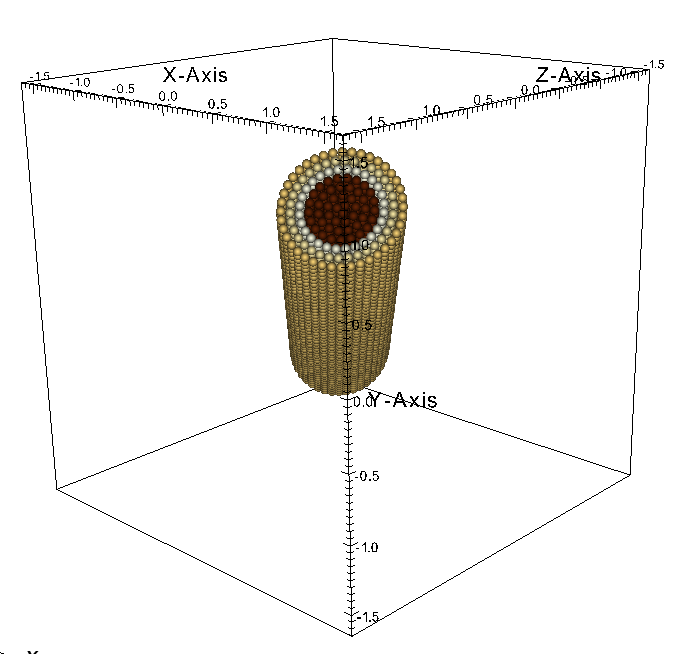
\includegraphics[width=0.9\columnwidth]{FIGS/geometry/geom_smooth_cyl_solid.png}
  \captionof{figure}{A \Textsfc{smoothcyl} geometry object. Particle volumes vary with radius.}
\end{minipage}

\begin{minipage}{0.6\textwidth}
  A hollow \Textsfc{smoothcyl} can be created by specifying an additional
  \Textsfc{thickness} parameter.  The thickness is required to be smaller than
  the radius.  The particle and grid resolution should be chosen such that the thickness
  contains at least two layers of particles.
  \begin{lstlisting}[language=XML]
    <smoothcyl label="cyl smooth">
      <bottom>[ -1.0, -1.0, -1.0]</bottom>
      <top>[ 1.0, 1.0, 1.0]</top>
      <radius> 0.5 </radius>
      <thickness> 0.2 </thickness>
    </smoothcyl>
  \end{lstlisting}
\end{minipage}
\begin{minipage}{0.4\textwidth}
  \centering
  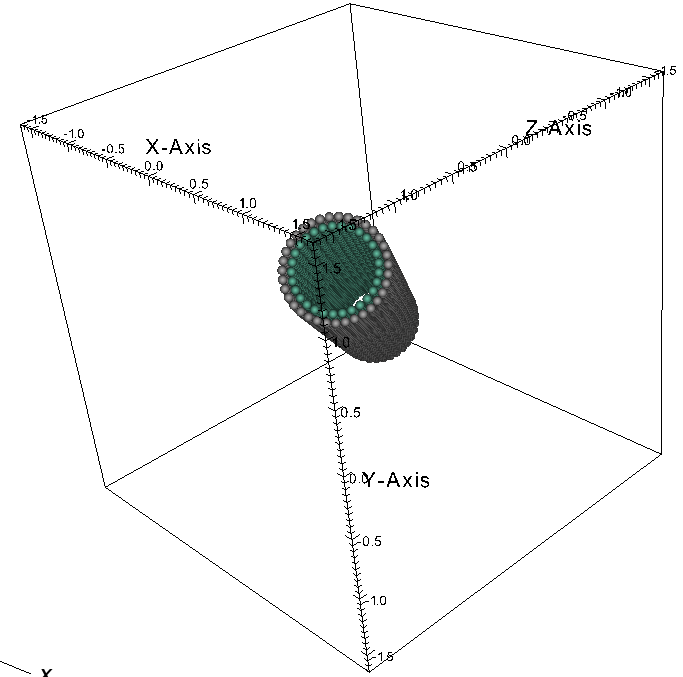
\includegraphics[width=0.9\columnwidth]{FIGS/geometry/geom_smooth_cyl_hollow.png}
  \captionof{figure}{A hollow \Textsfc{smoothcyl} geometry object.}
\end{minipage}

\begin{minipage}{0.6\textwidth}
  Endcaps can be added to the \Textsfc{smoothcyl} by specifying an additional
  \Textsfc{endcap thickness} parameter.  
  \begin{lstlisting}[language=XML]
    <smoothcyl label="cyl smooth">
      <bottom>[ -1.0, -1.0, -1.0]</bottom>
      <top>[ 1.0, 1.0, 1.0]</top>
      <radius> 0.5 </radius>
      <thickness> 0.2 </thickness>
      <endcap_thickness> 0.4 </endcap_thickness>
    </smoothcyl>
  \end{lstlisting}
\end{minipage}
\begin{minipage}{0.4\textwidth}
  \centering
  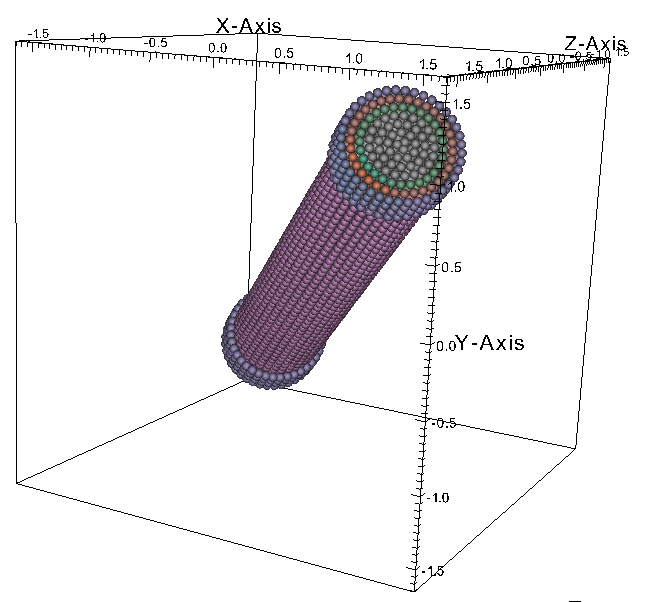
\includegraphics[width=0.9\columnwidth]{FIGS/geometry/geom_smooth_cyl_hollow_endcap.png}
  \captionof{figure}{A hollow \Textsfc{smoothcyl} with endcaps geometry object.}
\end{minipage}

\begin{minipage}{0.6\textwidth}
  Partial sectors of a \Textsfc{smoothcyl} can also be modeled by specifying \Textsfc{arc}
  information.  The start angle and arc angle default to 0 and 360 and have to be specified
  in degrees.
  The number of particles between \Textbfc{arc\_start} and \Textbfc{arc\_angle}
  is determined individually for each ring of particles by
  attempting to keep particle spacings approximately equal in the radial
  and angular directions, and thus particle volumes approximately
  constant.
  \begin{lstlisting}[language=XML]
    <smoothcyl label="cyl smooth">
      <bottom>[ -1.0, -1.0, -1.0]</bottom>
      <top>[ 1.0, 1.0, 1.0]</top>
      <radius> 0.5 </radius>
      <thickness> 0.2 </thickness>
      <endcap_thickness> 0.2 </endcap_thickness>
      <arc_start_angle_degree> 30 </arc_start_angle_degree>
      <arc_angle_degree> 90 </arc_angle_degree>
    </smoothcyl>
  \end{lstlisting}
\end{minipage}
\begin{minipage}{0.4\textwidth}
  \centering
  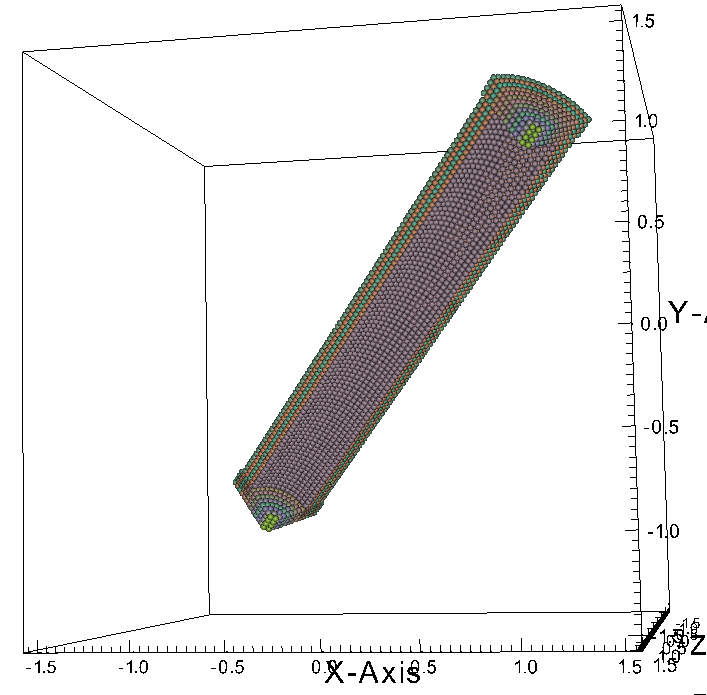
\includegraphics[width=0.9\columnwidth]{FIGS/geometry/geom_smooth_cyl_hollow_endcap_arc.png}
  \captionof{figure}{A partial hollow \Textsfc{smoothcyl} with endcaps.}
\end{minipage}

\begin{NoteBox}
Multiple \Textsfc{smoothcyl} geometries within a \Textbfc{\textless geom\_object\textgreater} 
tag are not
discretized using a body fit particle distribution as described here
(rather the default discretization scheme is used).  This will be
fixed eventually, at which point it may be possible to create more
general endcaps using unions of \Textsfc{smoothcyl}.
\end{NoteBox}

\subsection{Triangulated surface}
\Textsfc{tri} is a tag for describing a triangulated surface.
The name tag specifies the file name to use for reading in the
triangulated surface description and the points file.  The
triangulated surface (\Textbfc{file\_name.tri}) contains a list of integers
describing the connectivity of points specified in \Textbfc{file\_name.pts}.
Here is an excerpt from a tri file and a points file:

\begin{lstlisting}[backgroundcolor=\color{background}]
Triangulated file

1 39 41
1 41 38
38 41 42
. . .

Points file

0 0.03863 -0.005
0.35227 0.13023 -0.005
0.00403479 0.0296797 -0.005
. . .
\end{lstlisting}
The Mach 2 Wedge example in Section~\ref{Sec:MPMICE_EXAMPLES} depicts usage of
this option.

\subsection{Specifying particle locations directly}
In addition to the above, it is also possible in MPM simulations to describe
geometry by providing a file containing a series of particle locations.  These
can be in either ASCII or binary format.  In addition, it is also possible to
provide initial data for certain variables on the particles, including
volume, temperature, external force, fiber direction (used in material models
with transverse isotropy) and velocity.  The following is an example in which
external force and fiber direction are specified:
\begin{lstlisting}[language=XML]
          <file>
              <name>LVcoarse.pts</name>
              <var>p.externalforce</var>
              <var>p.fiberdir</var>
          </file>
\end{lstlisting}
where the text file \Textsfc{LVcoarse.pts} looks like:
\begin{lstlisting}[backgroundcolor=\color{background}]
0.0385 0.0335 0.0015 0 0 0 0.248865 -0.0593421 -0.966718
0.0395 0.0335 0.0015 0 0 0 0.254892 -0.0220365 -0.966718
0.0405 0.0335 0.0015 0 0 0 0.267002 0.0197728 -0.963493
0.0415 0.0335 0.0015 0 0 0 0.261177 0.0588869 -0.963493
	.
	.
	.
\end{lstlisting}
Because these files can be arbitrarily large, an additional preprocessing step
must be taken before issuing the \Textsfc{vaango} command.
\Textsfc{pfs} for \Textsfc{Particle File Splitter} is a utility that splits the
data in the \Textsfc{.pts} file into a series of files
(\Textsfc{file.pts.0, file.pts.1,}, etc), one for each
patch.  By doing this, each processor needs only read in the data for the
patches that it contains, rather than each processor reading in the entire file,
which can be hard on the file system.  Note, that this step is required,
even if only using a single patch, and must be reissued any time the patch
configuration is changed.  Usage of this utility, which is compiled
into the \Textsfc{StandAlone/tools/pfs} directory, is:
\begin{lstlisting}[backgroundcolor=\color{background}]
   pfs input.ups
\end{lstlisting}

\subsection{Using image data to create particles}
One final option is available for initializing particle positions in MPM
simulations, and that is through the use of three dimensional image data,
such as might be collected via CT scans or confocal microscopy.  The image data are 
provided as 8-bit raw files, and usage in the input file is given as:
\begin{lstlisting}[language=XML]
        <image>
          <name>spheres.raw</name>
          <res>[1600, 1600, 1600]</res>
          <threshold>[1, 25]</threshold>
        </image>
        <file>
          <name>spheres.pts</name>
          <format>bin</format>
        </file>
\end{lstlisting}
The \Textsfc{\textless image\textgreater} section gives the name of the file, the resolution, in pixels,
in the various coordinate directions, and threshold range.  Particles will be
generated at voxels within the specified range.  The \Textsfc{\textless file\textgreater}
section is the same as that described above.  A different preprocessing utility
is provided when using image data (for the same reasons described previously).
Usage is as follows:
\begin{lstlisting}[backgroundcolor=\color{background}]
   pfs2 -b input.ups
\end{lstlisting}
The \Textbfc{-b} flag indicates that binary \Textsfc{spheres.pts.\#} files will be created, which
saves considerable disk space when performing large simulations.

